\section{Deep Reinforcement Learning}

"Playing Atari with Deep Reinforcement Learning" \cite{mnih2013playing} and "Deep Reinforcement Learning: Pong from Pixels" \cite{karpathy2016deep} show how applying Deep Reinforcement Learning for the game of pong leads to the best results.

RISOLVE I PROBLEMI\\

The policy function, or policy network, used to decide what to do based on the current state, is a fully connected neural network with n hidden layers, which is why this method is called Deep RL. In the papers frame image of the game is taken as input, in which each pixel corresponds to a single input neuron, and returns a number between 0 and 1 which can be seen as the probability to win with a given action (e.g. left). If the number is greater than 0.5 we go to the left, otherwise we go to the right. If it is 0.5, a random choice is made. To do this, the output neuron has a sigmoid function \cite{mnih2013playing}\cite{karpathy2016deep}.
Since politics generates probability, this politics is stochastic.

\begin{figure}[ht]
    \centering
    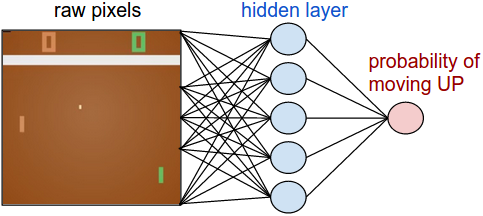
\includegraphics[scale=0.4]{images/DRL_network.png}
    \caption{Simple image of the policy network of an Deep RL system.}
    \label{fig:DRL_network}
\end{figure}

This can also be easily applied to inputs of a different nature, such as vectors representing the position of the ball, the direction, the position of the paddles, etc.